\documentclass{article}
\usepackage{amssymb,amsmath}
\usepackage{graphicx}
\title{FMR analysis with LLGS equation}

\begin{document}
\maketitle
\begin{abstract}

Ferromagnetic resonance measurements via BLS on microscopic Permalloy/Cu/Pt multilayer structures can be analysed in the framework of the LLG equation with variable Gilbert damping parameter $\alpha$. When so viewed, $\alpha$ scales linearly with current, capturing the broadening/narrowing of the resonance curve with increasing/decreasing current, respectively. At the same time, experimental results show that (LLG + variable $\alpha$) does not accurately explain the variation of the resonance peak amplitude with current, even when normalized to $I$ = 0 values. The discrepancy is termed ``amplification."

Moreover, a simple analysis based on the LLG equation with a ``Slonczewski" term (LLGS equation) suggests that these experimental results are also not captured by LLGS.
\end{abstract}
\section{Preliminaries}
We consider the following form of the LLGS,
\begin{equation}\label{LLGS}
\frac{d\vec{M}}{dt} = -\gamma \vec{M} \times \mu_{0} \vec{H}_{eff} + \frac{\alpha}{M_{s}} \vec{M} \times \frac{d\vec{M}}{dt} + \frac{\beta}{M_{s}^2}\vec{M} \times (\vec{M} \times \hat{z}).
\end{equation}
The effective field comprises the static external applied field $\vec{H}_{e}$, the dipolar field $\vec{H}_{dip} = - \overleftrightarrow{N} \vec{M}$, and the microwave field $\vec{h}_{e}$. 
We decompose $\vec{M}$ and $\vec{H}_{eff}$ into static and time-varying contributions, $\vec{M} = \vec{M}_{0} + \vec{m}_{\sim}$ and $\vec{H}_{eff} = \vec{H}_{0} + \vec{h}_{\sim}$. 
Note that $\vec{h}_{\sim} = \vec{h}_{e} - \overleftrightarrow{N} \vec{m}_{\sim}$ and $\vec{H}_{0} = \vec{H}_{e} - \overleftrightarrow{N} \vec{M}_{0}$. 
Additionally, we assume $\| \vec{h}_{\sim} \| \ll \| \vec{H}_{0} \|$ and $\| \vec{m}_{\sim} \| \ll \| \vec{M}_{0} \|$. 
Linearizing \eqref{LLGS} yields:
\begin{align}\label{LLGSlin}
\frac{d\vec{m}_{\sim}}{dt} = &- \gamma \mu_{0} \vec{M}_{0} \times \vec{H}_{0} - \gamma \mu_{0} \vec{M}_{0} \times \vec{h}_{\sim} - \gamma \mu_{0} \vec{m}_{\sim} \times \vec{H}_{0} \nonumber \\
& + \frac{\alpha}{M_{s}} \vec{M}_{0} \times \frac{d\vec{m}_{\sim}}{dt} + \frac{\beta}{M_{s}^2} \vec{M}_{0} \times ( \vec{m}_{\sim} \times \hat{z} ).
\end{align}
The system is considered at equilibrium, therefore $\vec{M}_{0} \times \vec{H}_{0} = 0$. 
We assume harmonic excitation at frequency $\omega$ and harmonic response at $\omega$. 
We employ the method of complex amplitudes. 
The time-varying contributions to $\vec{M}$ and $\vec{H}_{eff}$ are then given by $\vec{h}_{\sim} = \Re [ \vec{h} e^{i \omega t} ]$ and $\vec{m}_{\sim} = \Re [ \vec{m} e^{i \omega t} ]$.
We rewrite \eqref{LLGSlin} for the complex amplitudes $\vec{h}$ and $\vec{m}$:
\begin{equation}\label{LLGSlincom}
i \omega \vec{m} = - \gamma \mu_{0} \vec{M}_{0} \times \vec{h} - \gamma \mu_{0} \vec{m} \times \vec{H}_{0} + \frac{\alpha}{M_{s}} \vec{M}_{0} \times i \omega \vec{m} + \frac{\beta}{M_{s}^2} \vec{M}_{0} \times ( \vec{m} \times \hat{z} ).
\end{equation}
We orient the $z$-axis to lie parallel to $\vec{H}_{0}$, hence $\vec{H}_{e} = (0,0,H_{e0})$. 
Inserting definitions for $\vec{H}_{0}$ and $\vec{h}$ yields:
\begin{align}\label{LLGlincom2}
i \omega \vec{m} = &- \gamma \mu_{0} \vec{M}_{0} \times \vec{h}_{e} + \gamma \mu_{0} \vec{M}_{0} \times \left( \overleftrightarrow{N} \vec{m} \right) - \gamma \mu_{0} \vec{m} \times \left[ \vec{H}_{e} - \overleftrightarrow{N} \vec{M}_{0} \right] \nonumber \\
&+ \frac{i \alpha \omega}{M_{s}} \vec{M}_{0} \times \vec{m} + \frac{\beta}{M_{s}^2} \vec{M}_{0} \times \left( \vec{m} \times \hat{z} \right).
\end{align}
We model the Py disk as an infinitely thin plate in the $yz$-plane. 
Hence, the demagnetization tensor has components $N_{11} = 4 \pi$, $N_{ij} = 0$ otherwise. 
We project \eqref{LLGlincom2} onto coordinate axes and solve for the components of the external susceptibility tensor $\overleftrightarrow{\chi}^{e}$, defined by $m_{i} = \sum_{j} \chi_{ij}^{e} h_{j}^{e}$. 
We define $\chi_{ij}^{e} = \chi_{ij}^{\prime} - i \chi_{ij}^{\prime\prime}$ where $\chi_{ij}^{\prime} , \chi_{ij}^{\prime\prime} \in \mathbb{R}$. 
For brevity, we have dropped the $e$ in $\overleftrightarrow{\chi}^{e}$; here and henceforth, we deal exclusively with the external susceptibility tensor. 
As components we find,
\begin{align}
\chi_{xx}^{\prime} &= \frac{\omega_{M}}{D}\left[ \omega_{H} J + 2 \left( \alpha \omega \right)^2 \omega_{1} - 2 \alpha K \omega^2 + \omega_{H} K^2 \right] \\
\chi_{xx}^{\prime\prime} &= \frac{\omega_{M} \omega}{D}\left[ 2 \alpha \omega_{1} \omega_{H} - \alpha J - 2 \omega_{H} K - \alpha K^2 \right] \\
\chi_{xy}^{\prime} &= \frac{\omega_{M}}{D} \left[ 2 \alpha \omega_{1} \omega^2 - 2 \omega^2 K - J K - K^3 \right] \\
\chi_{xy}^{\prime\prime} &= \frac{\omega_{M} \omega}{D} \left[ 2 K^2 - 2 \alpha \omega_{1} K - K^2 - J \right] \\
\chi_{yx}^{\prime} &= - \chi_{12}^{\prime} \\
\chi_{yx}^{\prime\prime} &= - \chi_{12}^{\prime\prime} \\
\chi_{yy}^{\prime} &= \frac{\omega_{M}}{D} \left[ \omega_{H} J + 4 \pi \omega_{M} J + 2 \left(\alpha \omega \right)^2 \omega_{1} - 2 \alpha K \omega^2 + K^2 \omega_{H} + 4 \pi \omega_{M} K^2 \right] \\
\chi_{yy}^{\prime\prime} &= \frac{\omega_{M} \omega}{D} \left[ 2 \alpha \omega_{1} \omega_{H} + 8 \pi \omega_{M} \alpha \omega_{1} - \alpha J - 2 \omega_{H} K - 8 \pi \omega_{M} K - \alpha K^2 \right] \\
\chi_{ij} &= 0, \text{ otherwise}.
\end{align}
For notational convenience, we have defined
\begin{align}
\omega_{M} &= \gamma \mu_{0} M_{s} \\
\omega_{H} &= \gamma \mu_{0} H_{e0} \\
\omega_{0} &= \sqrt{\omega_{H} \left( \omega_{H} + 4 \pi \omega_{M} \right)} \\
\omega_{1} &= \omega_{H} + 2 \pi \omega_{M} \\
J &= \omega_{0}^2 - \left( 1 + \alpha^2 \right) \omega^2 \\
K &= \frac{\beta}{M_{s}} \\
D &= J^2 + 4 \alpha^2 \omega^2 \omega_{1}^2 + K^4 + 2 K^2 J + 4 K^2 \omega^2 - 8 K \alpha \omega^2 \omega_{1}.
\end{align}
In order to ascertain pertinent values of the parameter $\beta$, we solve for the critical value $\beta_{c}$ at which Gilbert damping is compensated. 
We set $\vec{h}_{e} = (0,0,0)$ and project \eqref{LLGlincom2} onto coordinate axes. 
Enforcing compatibility of the resulting equations gives the frequency of ``free" oscillations $\omega_{f} = \omega_{f}^{\prime} + i \omega_{f}^{\prime\prime}$. 
Gilbert damping is compensated when $\omega_{f}^{\prime\prime} = 0$. 
So,
\begin{align}
\omega_{f}^{\prime\prime} &= \frac{1}{1 + \alpha^2} \left[ 2 \pi \omega_{M} \alpha + \alpha \omega_{H} - K \right] \\
\beta_{c} &= 2 \pi \alpha \omega_{M} M_{s} + \alpha \omega_{H} M_{s}.
\end{align}
We consider only excitation by the out-of-plane component of the microwave field, $h_{x}$, i.e. $\vec{h}_{e} = (h_{x},0,0)$. 
Therefore, the magnitude of the dynamic, out-of-plane magnetization is given by $\| m_{x} \|^2 = \| \chi_{xx} \|^2 h_{x}^2$.
\section{Results}
In (LLG + variable $\alpha$), calculating $\alpha$ by fitting to the linewidth of the experimental curves results in incorrect prediction of the (normalized) peak amplitude.
We search for qualitatively different behavior in LLGS.

We calculate the peak amplitude and linewidth of $\| \chi_{xx} \|^2$ in two cases. 
First, we set $\alpha$ to its value determined from the resonance curve with no applied current, $\alpha = 0.011$, and vary $\beta$ in the range $\left[ - \beta_{c}, \beta_{c} \right]$.
Thereby, we regard $\alpha$ as intrinsic and use $\beta$ to model the effect of applied current.
Second, we set $\beta = 0$ and vary $\alpha$ in the range $\left[0.001, 0.021 \right]$.
This merely reproduces the results of (LLG + variable $\alpha$).
The resultant plot appears in Fig. \ref{fwhm_ampl} and as a log-log graph in Fig. \ref{fwhm_ampl_log}.
\begin{figure}
  \centering
  \includegraphics[angle=-90,width=100mm]{fwhm_ampl.eps}
  \caption{Peak amplitude of $\| \chi_{xx} \|^2$ as a function of linewidth. \label{fwhm_ampl}}
\end{figure}

\begin{figure}
  \centering
  \includegraphics[angle=-90,width=100mm]{fwhm_ampl_log.eps}
  \caption{Peak amplitude of $\| \chi_{xx} \|^2$ as a function of linewidth, log-log plot. \label{fwhm_ampl_log}}
\end{figure}

From fits to data, we find $A \propto \frac{1}{\Delta f^2}$ where $A$ is the peak amplitude and $\Delta f$ the linewidth, for both cases.
There is no qualitative difference on the resonance curve between varying $\alpha$ or $\beta$.

Using experimental data, and values attained from analysis with (LLG + variable $\alpha$), we can calculate $\beta$ as a function of current and the normalized peak amplitude as a function of current.

First, we calculate the the linewidth of the resonance curve as a function of $\beta$ for various values of the effective magnetization taken from experiment with analysis via (LLG + variable $\alpha$), see Fig. \ref{linewidth_beta}.

\begin{figure}
  \centering
  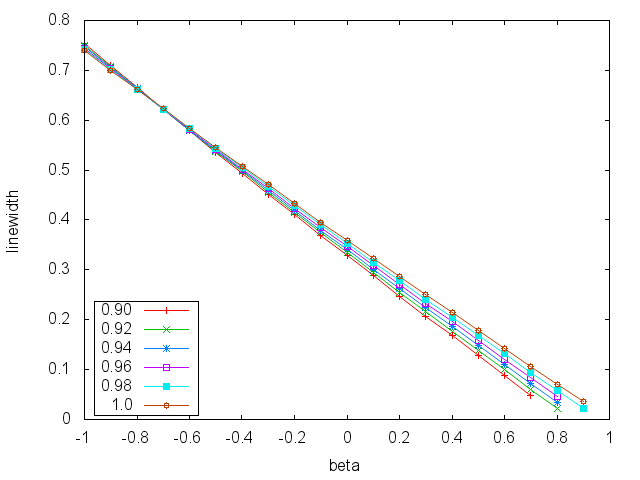
\includegraphics[angle=0,width=100mm]{linewidth_beta.png}
  \caption{Linewidth of $\| \chi_{xx} \|^2$ as a function of $\beta$, for several effective magnetizations. The horizontal axis is scalged to $\beta_{c}$ for effective magnetization equal to zero-current value measured in experiment. Linewidth plotted in GHz. \label{linewidth_beta}}
\end{figure}

Since the linewidth is a monotonically decreasing function of $\beta$ for all effective magnetizations, we can invert the curves to find $\beta$ as a function of linewidth and, therefore, $\beta$ as a function of current. 
We interpolate the inverted curves and find $\beta$ for the experimentally measured linewidths, yielding $\beta \left( I \right)$.
We find that $\beta$ approximately linearly decreases with increasing current, see Fig. \ref{current_beta_dc}.

\begin{figure}
  \centering
  \includegraphics[angle=-90,width=100mm]{current_beta_dc.eps}
  \caption{$\beta$ as a function of current. \label{current_beta_dc}}
\end{figure}

Lastly, we use these values of $\beta$ to calculate the normalized peak amplitude of the resonance curves.
Just as in (LLG + variable $\alpha$), we do not observe agreement between the calculated normalized peak amplitude and that observed in experiment. 
Amplification remains, see Fig. \ref{amplification_good}.

\begin{figure}
  \centering
  \includegraphics[angle=-90,width=100mm]{amplification_good.eps}
  \caption{Normalized peak amplitude of $\| \chi_{xx} \|^2$ as a function of current, alongside experimental values. \label{amplification_good}}
\end{figure}

\end{document}
In theory, as well as in experiment, the resonance curves of the magnitude of the magnetization as a function of frequency are nearly Lorentzian.
Therefore, the integral over these curves is well-approximated by the peak amplitude of the curve times its linewidth.